\documentclass[11pt]{amsart}
%\pagestyle{empty} 
\setlength{\topmargin}{-0.4in} % usually -0.25in
\addtolength{\textheight}{1.4in} % usually 1.25in
\addtolength{\oddsidemargin}{-0.6in}
\addtolength{\evensidemargin}{-0.6in}
\addtolength{\textwidth}{1.4in} %\setlength{\parindent}{0pt}

% macros
\usepackage{amssymb,xspace,verbatim}

\usepackage[pdftex, colorlinks=true, plainpages=false, linkcolor=black, citecolor=red, urlcolor=red]{hyperref}

\usepackage[final]{graphicx}
\newcommand{\regfigure}[3]{\includegraphics[height=#2in,width=#3in]{#1.eps}}

\newtheorem*{thm}{Theorem}
\newtheorem*{lem}{Lemma}

\usepackage{alltt}
\usepackage{fancyvrb}

\newcommand{\CC}{{\mathbb{C}}}
\newcommand{\RR}{{\mathbb{R}}}

\newcommand{\bb}{\mathbf{b}}
\newcommand{\bbf}{\mathbf{f}}
\newcommand{\br}{\mathbf{r}}
\newcommand{\bu}{\mathbf{u}}
\newcommand{\bv}{\mathbf{v}}
\newcommand{\bx}{\mathbf{x}}
\newcommand{\by}{\mathbf{y}}

\newcommand{\bzero}{\mathbf{0}}

\newcommand{\eps}{\epsilon}
\newcommand{\lam}{\lambda}

\newcommand{\ip}[2]{\mathrm{\left<#1,#2\right>}}
\newcommand{\erf}{\operatorname{erf}}

\newcommand{\Span}{\operatorname{span}}
\newcommand{\rank}{\operatorname{rank}}
\newcommand{\range}{\operatorname{range}}
\newcommand{\Null}{\operatorname{null}}

\newcommand{\cond}{\operatorname{cond}}

\renewcommand{\Re}{\operatorname{Re}}

\newcommand{\Matlab}{\textsc{Matlab}\xspace}
\newcommand{\Octave}{\textsc{Octave}\xspace}
\newcommand{\pylab}{\textsc{pylab}\xspace}

\newcommand{\mfile}[2]{
\bigskip
\begin{quote}
\medskip
\VerbatimInput[frame=single,framesep=3mm,label=\fbox{\normalsize \textsl{\,#1\,}},fontfamily=courier,fontsize=\scriptsize]{#2}
\medskip
\end{quote}
}

\DefineVerbatimEnvironment{mVerb}{Verbatim}{numbersep=2mm,
frame=lines,framerule=0.1mm,framesep=2mm,xleftmargin=4mm,fontsize=\footnotesize}


\newcommand{\prob}[1]{\bigskip\noindent\large \textbf{#1.} \normalsize}
\newcommand{\probpts}[2]{\bigskip\noindent\large \textbf{#1} \normalsize \,(\emph{#2})\,}
\newcommand{\ppart}[1]{\quad \textbf{#1)} }
\newcommand{\epart}[1]{\medskip\noindent\textbf{#1)}}


\begin{document}
\noindent \scriptsize Math 615 NADE (Bueler) \hfill 15 February 2023

\bigskip
\Large\textbf{\centerline{Solutions to Assignment \# 3}} \normalsize

\medskip
\begin{center}
\emph{The point value of each Problem is given below.  The total was XX points.}
\end{center}

\thispagestyle{empty}

\probpts{P12}{5 pts per part}  \ppart{a} I wrote the following code:

\mfile{richardson.m}{../richardson.m}

Running it as follows generates $x_3$ on slide 5 as requested:
\begin{mVerb}
>> A = [2 1 0; 0 2 1; 1 0 3];  b = [2 1 4]';  x0 = zeros(3,1);
>> z = richardson(A,b,x0,3,1/5)
z =
  0.72800
  0.08800
  1.09600
\end{mVerb}

\epart{b}  Based on the plot of spectral radii $\rho(I-\omega A)$ on slide 10, for the LS1 matrix the preferred value for $\omega$ is $0.4$.

And I interpret ``8 digit accuracy'' as $\|x_N-x\|_2 < 10^{-8}$ where $x=[1\,0\,1]^\top$ is the known exact solution.  For the three values of $\omega$, I wrote quick loops to stop at the first $N$ satisfying the criterion:
\begin{mVerb}
>> x = A \ b;
>> for N=1:100, if norm(richardson(A,b,x0,N,0.4) - x) < 1.0e-8, N, break, end, end
N =                   22
>> for N=1:100, if norm(richardson(A,b,x0,N,0.1) - x) < 1.0e-8, N, break, end, end
N =                   97
>> for N=1:100, if norm(richardson(A,b,x0,N,0.5) - x) < 1.0e-8, N, break, end, end
N =                   61
\end{mVerb}
We see that $\omega=0.4$ does indeed give faster convergence than $\omega=0.1,0.5$, and that the figure on slide 10 does a reasonable job of predicting what we see.

\medskip
\noindent
\emph{Comment.}  Other standards for ``8 digit accuracy'' are reasonable, but your method should be stated.


\clearpage \newpage
\probpts{P13}{5 pts per part}  \ppart{a}  I wrote these two codes:

\mfile{jacobi.m}{../jacobi.m}

\mfile{gs.m}{../gs.m}

In both codes, \texttt{noti} is a list of indices not equal to $i$:
    $$\text{\texttt{noti}} = \{1,2,\dots,i-1,i+1,\dots,m\} = \{j\,\big|\,j\neq i\}.$$

In \texttt{jacobi} we need to compute the whole \texttt{xnew} iterate $x_{k+1}$ before we can throw away the old vector $x_k$.  Thus there must be storage for both vectors.  However, \texttt{gs} is strictly simpler: we update entries of $x$ in sequence, immediately using the entries that have just been set.  Thus \texttt{gs} is a shorter code than \texttt{jacobi}, and uses less memory.

\medskip
\noindent
\emph{Comment.}  Jacobi \emph{parallelizes} better than Gauss-Seidel even though it uses a bit more memory and is slower (i.e.~requires more iterations to converge).  Both algorithms are in common use, but typically as parts of other algorithms and not as stand-alone solves.

\epart{b}  I get $23$ iterations for Jacobi and $16$ for Gauss-Seidel:
\begin{mVerb}
>> for N=1:100, if norm(jacobi(A,b,x0,N) - x) < 1.0e-8, N, break, end, end
N =                   23
>> for N=1:100, if norm(gs(A,b,x0,N) - x) < 1.0e-8, N, break, end, end
N =                   16
\end{mVerb}

Note that Gauss-Seidel uses fewer iterations than the optimized Richardson iteration above, and it does not require us to ``tune'' a parameter like $\omega$.  As a stand-alone solver, Gauss-Seidel is generally preferred over Richardson and Jacobi.

On LS2 Gauss-Seidel fails by explosion, as norms grow by almost an order of magnitude per iteration:
\begin{mVerb}
>> A = [1 2 3 0; 2 1 -2 -3; -1 1 1 0; 0 1 1 -1];  b = [7 1 1 3]';  x0 = [0 0 0 0]';
>> norm(gs(A,b,x0,5))
ans =    6.3010e+04
>> norm(gs(A,b,x0,50))
ans =    2.6132e+42
>> norm(gs(A,b,x0,500))
ans = NaN
\end{mVerb}

To explain the failure we compute the spectral radius $\rho((D-L)^{-1} U)$, because slide 14 says this should be smaller than one for convergence:
\begin{mVerb}
>> D = diag(diag(A));  L = -tril(A,-1);  U = -triu(A,+1);
>> max(abs(eig((D-L)\U)))
ans =  6.8541
\end{mVerb}
The explosion happens, at least asymptotically, as $\|x_k\| \approx C (6.85)^k$.


\probpts{P14}{15 pts}  \emph{The context.}  Let $M = D^{-1}(L+U)$ where $A=D-L-U$.  Here $D$ is diagonal, $L$ is strictly lower-triangular, and $U$ is strictly upper-triangular, and the nonzero entries of $D$ are the diagonal entries of $A$, while entries of $L,U$ are the negatives of the sub- and super-diagonal entries of $A$.  In these terms, the Jacobi iteration is $x_{k+1} = M x_k + D^{-1} b$ with constant vector $c=D^{-1} b$.  The convergence Lemma on slide 9 therefore says Jacobi iteration converges if and only if $\rho(M) < 1$.  We use these ideas to prove the following statement.

\medskip
If $A$ is strictly diagonally-dominant then the Jacobi iteration converges.

\begin{proof} Suppose $M v = \lambda v$ for $v\ne 0$.  We will show $|\lambda|<1$ so that, because $\lambda$ is an arbitrary eigenvalue of $M$, $\rho(M)<1$.

Choose the largest-magnitude entry $v_i$ of $v$, so that $|v_i| \ge |v_j|$ for all $j$.  Note in particular that $|v_i| > 0$ because $v$ is not the zero vector.  Because $A$ is strictly diagonally-dominant, for each $i$ we know that $|a_{ii}| > \sum_{j\ne i} |a_{ij}|$.  Then
\begin{align*}
|\lambda| |v_i| &= |(\lambda v)_i| = |(M v)_i| = \left|- a_{ii}^{-1} \left(\sum_{j>i} a_{ij} v_j + \sum_{j<i} a_{ij} v_j\right)\right| \\
  &\le |a_{ii}|^{-1} \left(\sum_{j>i} |a_{ij}| |v_j| + \sum_{j<i} |a_{ij}| |v_j|\right) \le |a_{ii}|^{-1} \left(\sum_{j>i} |a_{ij}| |v_i| + \sum_{j<i} |a_{ij}| |v_i|\right) \\
  &= |v_i| |a_{ii}|^{-1} \sum_{j\ne i} |a_{ij}| < |v_i| |a_{ii}|^{-1} |a_{ii}| = |v_i|.
\end{align*}
That is, $|\lambda| |v_i| < |v_i|$, and $|v_i|\ne 0$, so $|\lambda|<1$.

Since $\rho(M)<1$, by the Lemma on slide 9, the Jacobi iteration converges.
\end{proof}


\probpts{P15}{5 pts per part}  \ppart{a}  Based on the solution to \textbf{P10}, I wrote the following small modification of the code \texttt{steadyheat.m}:\footnote{See the Codes tab of the public course site.}

\mfile{bvpq.m}{bvpq.m}

\epart{b}  Note that, in manufacturing a solution, $f(x)$ is computed by plugging-in the exact $u(x)$ and simply differentiating etc.~as needed:
	$$f(x) = u''(x) - u(x) = \dots = \left(\frac{\pi^2}{4^2} + 1\right) \sin\left(\frac{\pi}{4} x\right) - 1$$
Now the \texttt{help bvpq} comments in \texttt{bvpq.m} show how to solve the suggested test case:
\begin{mVerb}
>> f = @(x) (pi^2/4^2 + 1) * sin((pi/4)*x) - 1;
>> [x,U] = bvpq(20,0,2,-1,f,1,0);
>> uexact = @(x) 1 - sin((pi/4)*x);
>> plot(x,U,'o',x,uexact(x),'-')
>> xlabel x,  legend('numerical','exact')
\end{mVerb}
This generates a figure showing the numerical solution for $m=20$ interior points, right on top of the exact solution.

But how accurate is it, really?  And as $h \to 0$ do we get the expected rate of convergence of the error norms $\|U^h - \hat U^h)\|$, where $\hat U_j^h = u(x_j)$?  This can be done by a loop at the command line, for $m$ equal to powers of 2, measuring the error norms, and then using \texttt{polyfit} to get the convergence rate:
\begin{mVerb}
>> m = 2.^(1:7);
>> for k = 1:7, [x,U] = bvpq(m(k),0,2,-1,f,1,0); err(k)=norm(U-uexact(x),'inf'); end 
>> p = polyfit(log(h),log(err),1)
p =
       1.9911      -4.8924
>> loglog(h,err,'o',h,exp(p(2) + p(1)*log(h)),'r:')
>> xlabel h, ylabel('|U - u_{exact}|')
>> text(0.1,0.001,'O(h^{1.99})','Color','r','FontSize',18)
\end{mVerb}
The convergence rate of $E^h = \|U^h - \hat U^h)\| = C h^{1.99}$ is essentially perfect for the expected errors $O(h^2)$.  The generated figure is below

\begin{center}
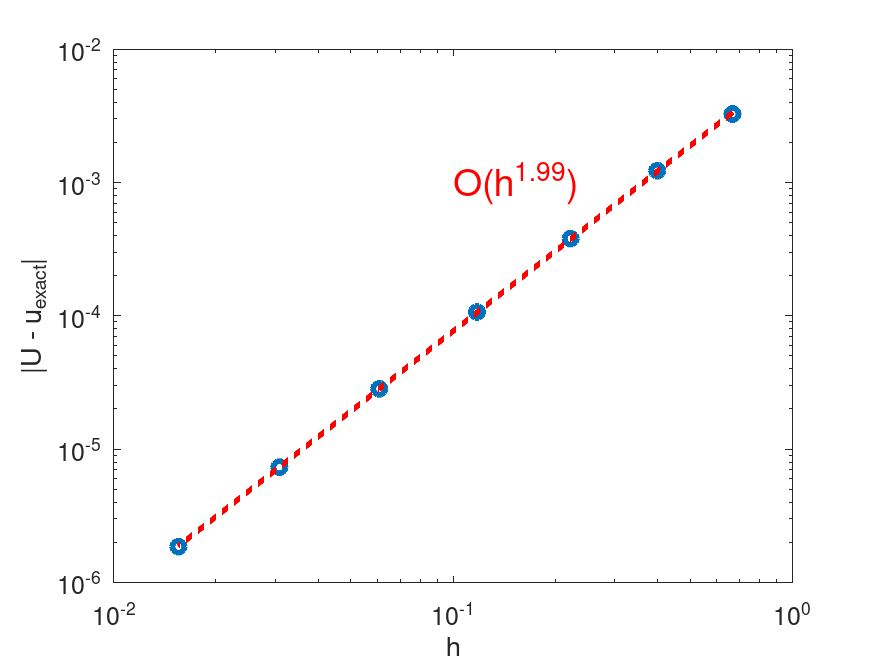
\includegraphics[width=0.6\textwidth]{bvpq.png}
\end{center}

\epart{c}  The matrix diagonal entries are
	$$a_{ii} = \frac{1}{h^2} (-2 + q h^2) = - \frac{2}{h^2} + q.$$
For every row except the first and last rows, the sum of the off-diagonal entries is
	$$\sum_{j\ne i} = \frac{1}{h^2} + \frac{1}{h^2} = \frac{2}{h^2}.$$
SDD says
    $$\left|- \frac{2}{h^2} + q\right| > \frac{2}{h^2}$$
in this case.  As $h\to \infty$ the terms with $h^2$ in the denominator dominate, so SDD cannot occur if $q\ge 0$.  However, if $q<0$ then the inequality becomes
    $$\frac{2}{h^2} + |q| > \frac{2}{h^2}$$
which simply says $q<0$.  That is, $A^h$ is SDD for all $h$ if and only if $q<0$.

\medskip
\noindent
\emph{Comment.}  The ODE $u''(x) + q u(x) = f(x)$ is sometimes called the \emph{good Helmholz} equation when $q<0$, and \emph{bad Helmholz} if $q>0$.  The invertibility of $A^h$ in the $q<0$ cases is one way to explain this language.

\epart{d}  Not due and not graded.  Discussed in class.


\clearpage\newpage
\probpts{P16}{5 pts}  If $f(x)$ is a scalar function then the Jacobian is the ordinary derivative $J(x) = f'(x)$, thus the equations (8), (9) from the slides are simply
\begin{align*}
f'(x_k) s &= -f(x_k) \\
x_{k+1} &= x_k + s
\end{align*}
Solving the first for $s$, by assuming the Jacobian is invertible, i.e.~assuming $f'(x_k)\ne 0$, and substituting in the second, we get the memorized equation $x_{k+1} = x_k - f(x_k) / f'(x_k)$.



FIXME check next

\probpts{P17}{5 pts per part}  The sketchs are omitted, but they show a sphere of radius 2, a corrugated surface, and a parabolic trough, respectively.  The solutions to the first two equations form a wavy line on the sphere, and going around the sphere.  The surface of the third equation (the parabolic trough) intersects this wavy line in two points.  Thus we expect two solutions, one with $y>0$ and one with $y<0$.  Any simultaneous solution $(x,y,z)$ is on the sphere and thus inside the cube centered at the origin with side length 4.  But it has $|x|\le 1$ by the second equation and $z\ge 0$ by the third equation.  Thus $(x,y,z)$ is inside $[-1,1]\times [-2,2] \times [0,2]$.

\epart{b}  The first step is to put the system in the form $\bbf(\bx)=\bzero$.  We have $f_1(x) = x_1^2 + x_2^2 + x_3^2 - 4$, $f_2(x) = x_1 - \cos(\pi x_2)$, and $f_3(x) = x_3 - x_2^2$ as the components of the vector $\bf(\bx)$, so
  $$\bbf(\bx) = \begin{bmatrix} x_1^2 + x_2^2 + x_3^2 - 4 \\ x_1 - \cos(\pi x_2) \\ x_3 - x_2^2 \end{bmatrix} \qquad \text{and} \qquad J(\bx) = \begin{bmatrix} 2 x_1 & 2 x_2 & 2 x_3 \\ 1 & \pi \sin(\pi x_2) & 0 \\ 0 & -2 x_2 & 1 \end{bmatrix}.$$
I put these functions $\bbf(\bx)$ and $J(\bx)$ into the script:

\mfile{newtonex.m}{newtonex.m}

The results of the run
\begin{mVerb}
>> newtonex([-1 1 1],6)
\end{mVerb}
include Figure 1.  The solution itself is
    $$\bx_+^* = (-0.856360744261663, 1.172720052019146, 1.375272320407789).$$
The other solution $\bx_-^*$ is the same except that $x_2$ is opposite in sign.  It can be found by
\begin{mVerb}
>> newtonex([-1 -1 1],6)
\end{mVerb}

\begin{figure}[ht]
FIXME %\includegraphics[height=2.6in,keepaspectratio=true]{figs/a2p5newton}
\caption{Residual norm ($y$-axis) crashes downward in Newton's method.}
\end{figure}


\end{document}

